\documentclass[tikz,border=3pt]{standalone}
\usepackage[utf8]{inputenc}
\usepackage[T1]{fontenc}
\usepackage{lmodern}
\renewcommand{\familydefault}{\sfdefault}
\usepackage{sansmath}\sansmath
\usepackage{chemfig}
\usepackage{pgfplots}\pgfplotsset{compat=1.18,/pgf/number format/use comma,/pgf/number format/1000 sep={.}}
\usetikzlibrary{arrows.meta,calc,positioning,decorations.pathmorphing,patterns}
% paleta del sitio
\definecolor{nar}{HTML}{E8680C}\definecolor{narc}{HTML}{FFB35C}\definecolor{hielo}{HTML}{FFF3E8}
\definecolor{tinta}{HTML}{1D1D1F}\definecolor{gris}{HTML}{6E6E73}\definecolor{lila}{HTML}{7C5CF0}
\definecolor{azul}{HTML}{2F6FD6}\definecolor{menta}{HTML}{17A673}\definecolor{coral}{HTML}{E8342A}
\begin{document}
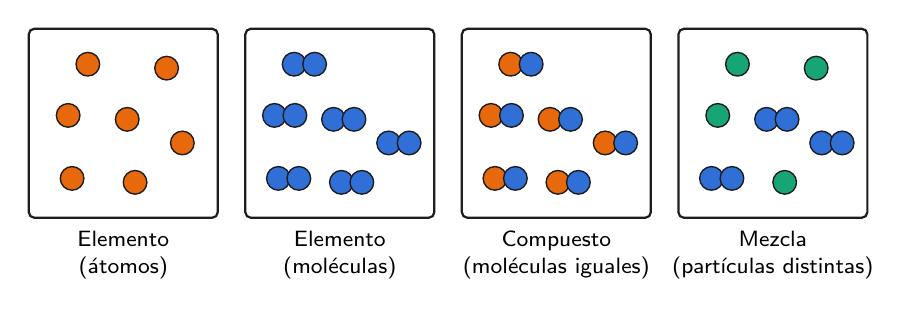
\begin{tikzpicture}[font=\small]
\draw[tinta,thick,fill=white,rounded corners=2pt] (0,0) rectangle (2.4,2.4);
\fill[nar,draw=tinta,line width=0.5pt] (0.55,0.5) circle (0.15);
\fill[nar,draw=tinta,line width=0.5pt] (1.35,0.45) circle (0.15);
\fill[nar,draw=tinta,line width=0.5pt] (1.95,0.95) circle (0.15);
\fill[nar,draw=tinta,line width=0.5pt] (0.5,1.3) circle (0.15);
\fill[nar,draw=tinta,line width=0.5pt] (1.25,1.25) circle (0.15);
\fill[nar,draw=tinta,line width=0.5pt] (0.75,1.95) circle (0.15);
\fill[nar,draw=tinta,line width=0.5pt] (1.75,1.9) circle (0.15);
\node[below,align=center,font=\footnotesize] at (1.2,-0.05) {Elemento\\(átomos)};
\draw[tinta,thick,fill=white,rounded corners=2pt] (2.75,0) rectangle (5.15,2.4);
\fill[azul,draw=tinta,line width=0.5pt] (3.17,0.5) circle (0.15);
\fill[azul,draw=tinta,line width=0.5pt] (3.43,0.5) circle (0.15);
\fill[azul,draw=tinta,line width=0.5pt] (3.97,0.45) circle (0.15);
\fill[azul,draw=tinta,line width=0.5pt] (4.23,0.45) circle (0.15);
\fill[azul,draw=tinta,line width=0.5pt] (4.57,0.95) circle (0.15);
\fill[azul,draw=tinta,line width=0.5pt] (4.83,0.95) circle (0.15);
\fill[azul,draw=tinta,line width=0.5pt] (3.12,1.3) circle (0.15);
\fill[azul,draw=tinta,line width=0.5pt] (3.38,1.3) circle (0.15);
\fill[azul,draw=tinta,line width=0.5pt] (3.87,1.25) circle (0.15);
\fill[azul,draw=tinta,line width=0.5pt] (4.13,1.25) circle (0.15);
\fill[azul,draw=tinta,line width=0.5pt] (3.37,1.95) circle (0.15);
\fill[azul,draw=tinta,line width=0.5pt] (3.63,1.95) circle (0.15);
\node[below,align=center,font=\footnotesize] at (3.95,-0.05) {Elemento\\(moléculas)};
\draw[tinta,thick,fill=white,rounded corners=2pt] (5.5,0) rectangle (7.9,2.4);
\fill[nar,draw=tinta,line width=0.5pt] (5.92,0.5) circle (0.15);
\fill[azul,draw=tinta,line width=0.5pt] (6.18,0.5) circle (0.15);
\fill[nar,draw=tinta,line width=0.5pt] (6.72,0.45) circle (0.15);
\fill[azul,draw=tinta,line width=0.5pt] (6.98,0.45) circle (0.15);
\fill[nar,draw=tinta,line width=0.5pt] (7.32,0.95) circle (0.15);
\fill[azul,draw=tinta,line width=0.5pt] (7.58,0.95) circle (0.15);
\fill[nar,draw=tinta,line width=0.5pt] (5.87,1.3) circle (0.15);
\fill[azul,draw=tinta,line width=0.5pt] (6.13,1.3) circle (0.15);
\fill[nar,draw=tinta,line width=0.5pt] (6.62,1.25) circle (0.15);
\fill[azul,draw=tinta,line width=0.5pt] (6.88,1.25) circle (0.15);
\fill[nar,draw=tinta,line width=0.5pt] (6.12,1.95) circle (0.15);
\fill[azul,draw=tinta,line width=0.5pt] (6.38,1.95) circle (0.15);
\node[below,align=center,font=\footnotesize] at (6.7,-0.05) {Compuesto\\(moléculas iguales)};
\draw[tinta,thick,fill=white,rounded corners=2pt] (8.25,0) rectangle (10.65,2.4);
\fill[azul,draw=tinta,line width=0.5pt] (8.67,0.5) circle (0.15);
\fill[azul,draw=tinta,line width=0.5pt] (8.93,0.5) circle (0.15);
\fill[menta,draw=tinta,line width=0.5pt] (9.6,0.45) circle (0.15);
\fill[azul,draw=tinta,line width=0.5pt] (10.07,0.95) circle (0.15);
\fill[azul,draw=tinta,line width=0.5pt] (10.33,0.95) circle (0.15);
\fill[menta,draw=tinta,line width=0.5pt] (8.75,1.3) circle (0.15);
\fill[azul,draw=tinta,line width=0.5pt] (9.37,1.25) circle (0.15);
\fill[azul,draw=tinta,line width=0.5pt] (9.63,1.25) circle (0.15);
\fill[menta,draw=tinta,line width=0.5pt] (9,1.95) circle (0.15);
\fill[menta,draw=tinta,line width=0.5pt] (10,1.9) circle (0.15);
\node[below,align=center,font=\footnotesize] at (9.45,-0.05) {Mezcla\\(partículas distintas)};

\end{tikzpicture}
\end{document}
